\documentclass[12pt, bachelor, substylefile = algo_title.rtx]{disser}

\usepackage[a4paper,
            left=1.5cm, right=1.5cm,
            top=2cm, bottom=2cm,
	 headsep=1cm, footskip=1cm]{geometry}
\usepackage[T2A]{fontenc}
\usepackage[utf8]{inputenc}
\usepackage[english]{babel}
\usepackage{amsmath, amsthm}
\usepackage{hyperref}
\usepackage{amsfonts}
%\usepackage{indentfirst}
\usepackage{xcite}
\usepackage{xr}
\usepackage{outlines}
\usepackage{mathtools}
\usepackage{subcaption}
%\usepackage{newtxtext,newtxmath}
\usepackage[final]{pdfpages}


\DeclarePairedDelimiter\ceil{\lceil}{\rceil}
\DeclarePairedDelimiter\floor{\lfloor}{\rfloor}
\newcommand{\Hyp}{\ensuremath{\mathbb{H}}}
\newcommand{\Pb}{\mathcal{P}}
\newcommand{\ME}{\mathbb{E}}
\newcommand{\med}{\mathbb{M}}
\newcommand{\Proba}{\mathbb{P}}
\newcommand{\VAR}{\mathbb{D}}
\newcommand{\varD}{\mathbf{D}}
\newcommand{\eps}{\varepsilon}
\newcommand{\varZ}{\mathbf{Z}}
\newcommand{\varV}{\mathbf{V}}
\newcommand{\varW}{\mathbf{W}}
\newcommand{\varY}{\mathbf{Y}}
\newcommand{\varX}{\mathbf{X}}
\newcommand{\varR}{\mathbf{R}}
\newcommand{\varS}{\mathbf{S}}
\newcommand{\varU}{\mathbf{U}}
\newcommand{\ind}{\mathbb{I}}
\newcommand{\Real}{\mathbb{R}}
\newcommand{\Sample}{\varV_1,\varV_2,\dots,\varV_m}
\newcommand{\Samplex}{\varX_1,\varX_2,\dots,\varX_n}
\DeclareMathOperator{\sign}{sign}

\newcommand{\specialcell}[2][c]{%
  \begin{tabular}[#1]{@{}c@{}}#2\end{tabular}}

\theoremstyle{definition}
\newtheorem{theorem}{Theorem}
\newtheorem{definition}{Definition}
\newtheorem{assumption}{Assumption}
\newtheorem{lemma}{Lemma}
\newtheorem{example}{Example}
\newtheorem{proposition}{Proposition}
\newtheorem{conseq}{Consequence}

\setcounter{tocdepth}{2}


\begin{document}

\institution{FEDERAL STATE AUTONOMOUS EDUCATIONAL INSTITUTION\\
OF HIGHER EDUCATION\\
ITMO UNIVERSITY
}
\title{Report on learning practice \#2}


\topic{\normalfont\scshape %
Analysis of multivariate random variables}
\author{Dmitry Grigorev,\\ Eugenia Khomenko,\\ Efim Podkovirkin,\\ Arina Syrchenko}

\city{St. Petersburg}
\date{2022}

\maketitle

\tableofcontents

\section{Data description}

Let $D$ is a subsample on size $n = 1000$ from modified dataset on Narvik roads. The features here are:

\begin{outline}
\1lat\_ — latitude
\1 lon\_ — longitude
\1 State\_ — word description of road state (1: 'dry', 2: 'moist', 3: 'wet', 4: 'icy', 5: 'snowy', 6: 'slushy')
\1 Ta\_mean,Ta\_min,Ta\_max — atmosphere temperature
\1 Tsurf\_mean,Tsurf\_min,Tsurf\_max — surface temperature
\1 Water\_mean,Water\_min,Water\_max — water layerw width (0 -- 3 $mm$)
\1 Speed\_mean,Speed\_min,Speed\_max — wind speed (in knots, $5\ knots \approx 9.3\ km/h$)
\1 Height\_mean,Height\_min,Height\_max — height of location above mean sea level
\1 Tdew\_mean,Tdew\_min,Tdew\_max — dew point ($Celsius$)
\1 Friction\_mean,Friction\_min,Friction\_max — friction value ( 0 -- 1, 0 means no friction)
\1 Date,Time, date\_time, FullDate — time and date
\1 Direction\_min,Direction\_max — wind direction ($degrees$)
\1 ClosestCity, location
\1 maxtempC,mintempC — day maximum and minimum of temperature ($Celsius$)
\1 totalSnow\_cm — total snowfall ($cm$)
\1 sunHour — passed sun energy in $Sun-Hours$ (A $Sun-Hour$ is "1000 watts of energy shining on 1 square meter of surface for 1 hour")
\1 uvIndex — ultraviolet index
\1 moon\_illumination — moon phase ($percents$)
\1 moonrise — time of Moon rise
\1 moonset — time of Moon set
\1 sunrise — time of Sun rise
\1 sunset — time of Sun set
\1 DewPointC — hourly dew point measurement ($Celsius$)
\1 FeelsLikeC — hourly Feels-like temperature ($Celsius$)
\1 HeatIndexC — hourly heat index ($Celsius$)
\1 WindChillC — hourly wind-chill index ($Celcius$) 
\1 WindGustKmph — hourly wind gust measure ($km/h$)
\1 cloudcover — hourly cloud cover index ($percents$)
\1 humidity — hourly humidity ($percents$)
\1 precipMM — hourly precipitation ($mm$)
\1 pressure — hourly atmosphere pressure ($mbar$)
\1 tempC — hourly atmosphere temperature ($Celsius$)
\1 visibility — hourly visibility (0--10, 0 means poor visibility)
\1 winddirDegree — hourly wind direction ($degrees$)
\1 windspeedKmph — hourly wind speed ($km/h$)
\end{outline}


\begin{figure}[!h]
\centering
   \begin{minipage}{0.7\textwidth}
     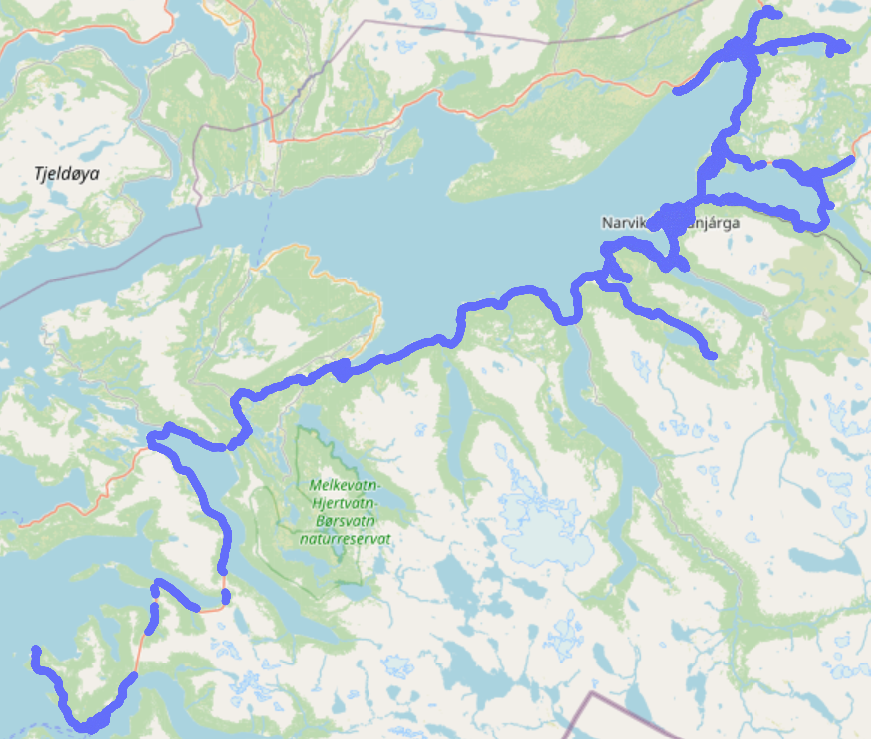
\includegraphics[width=\linewidth]{geography}
   \end{minipage}
\caption{Geography of the data}
\label{fig: }
\end{figure}

\section{Plotting a non-parametric estimation of PDF in form of a histogram and kernel
density function for MRV (or probability law in case of discrete MRV)}

Here one can observe histograms and KDE of density of Friction\_mean and DewPointC variables as an example. The first looks like bimodal distribution and this bimodality is explained by State\_: it is possible to separate Friction\_mean with respect to State\_ $<4$, State\_ $=4$, State\_ $>4$. We use this information further in analysis.

\begin{figure}[!h]
\centering
   \begin{minipage}{0.48\textwidth}
     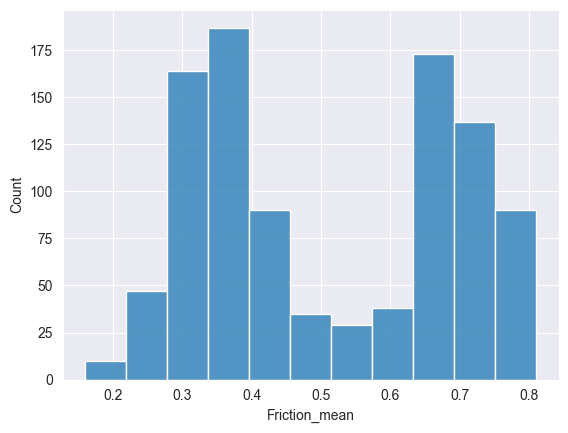
\includegraphics[width=.7\linewidth]{friction_hist}
	\label{fig: 1a}
   \end{minipage}\\
   \begin{minipage}{0.48\textwidth}
     \centering
     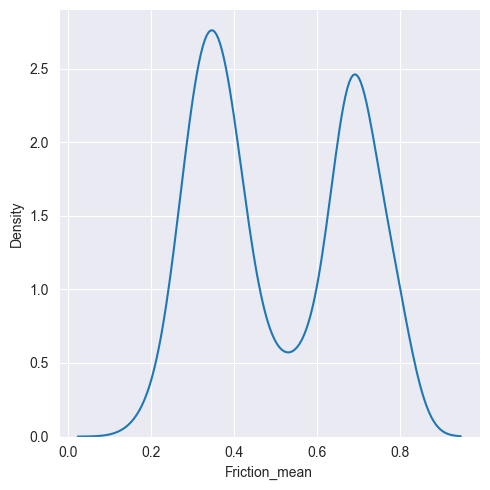
\includegraphics[width=.7\linewidth]{friction_kde}
	\label{fig: 1b}
   \end{minipage}\hfill
\begin{minipage}{0.48\textwidth}
     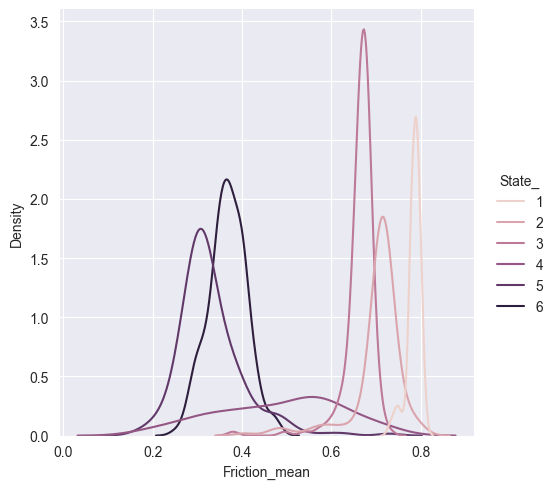
\includegraphics[width=.7\linewidth]{friction_kde1}
	\label{fig: 1c}
   \end{minipage}
\caption{Friction\_mean's histogram, KDE and KDE conditional on State\_}
\label{fig: 1}
\end{figure}

\begin{figure}[!h]
\centering
   \begin{minipage}{0.48\textwidth}
     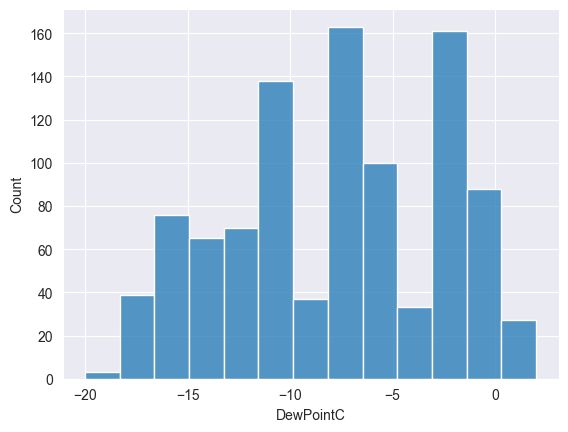
\includegraphics[width=.7\linewidth]{dewpoint_hist}
	\label{fig: 2a}
   \end{minipage}\\
   \begin{minipage}{0.48\textwidth}
     \centering
     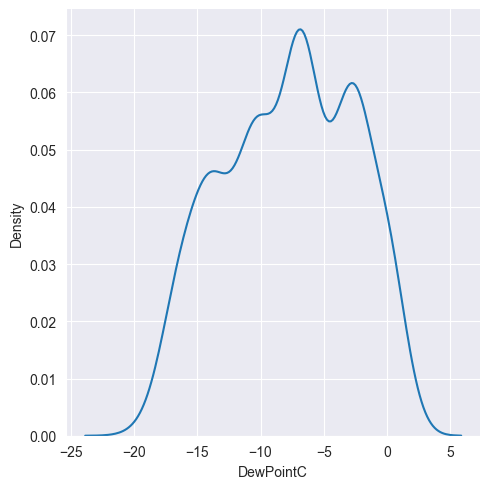
\includegraphics[width=.7\linewidth]{dewpoint_kde}
	\label{fig: 2b}
   \end{minipage}\hfill
\begin{minipage}{0.48\textwidth}
     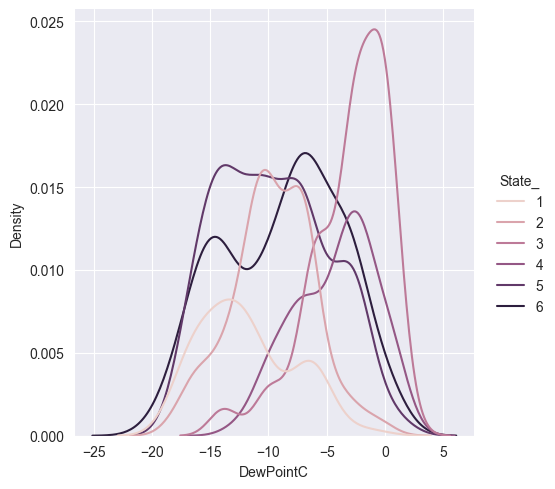
\includegraphics[width=.7\linewidth]{dewpoint_kde1}
	\label{fig: 2c}
   \end{minipage}
\caption{DewPointC's histogram, KDE and KDE conditional on State\_}
\label{fig: 2}
\end{figure}

Here visibility's distribution is also provided by both histogram and table. As one can see, the distribution is heavily focused on value 10.

\begin{figure}[!h]
\centering
   \begin{minipage}{0.7\textwidth}
     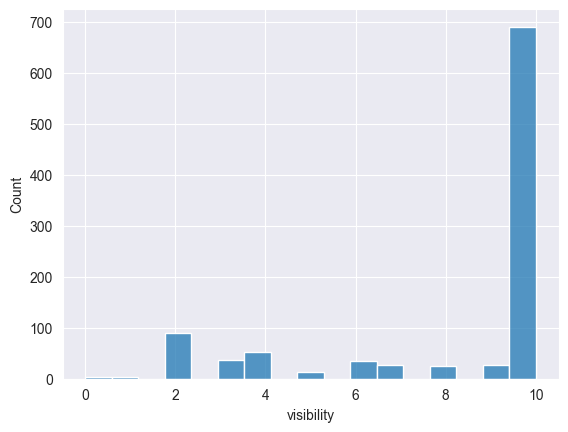
\includegraphics[width=\linewidth]{visibility_hist}
	\label{fig: 3a}
   \end{minipage}\\
\caption{visibility's histogram}
\label{fig: 3}
\end{figure}

Moreover, pair-plot for a subset of features is provided in figure \ref{fig: 4}.

\begin{figure}[!h]
\centering
   \begin{minipage}{0.9\textwidth}
     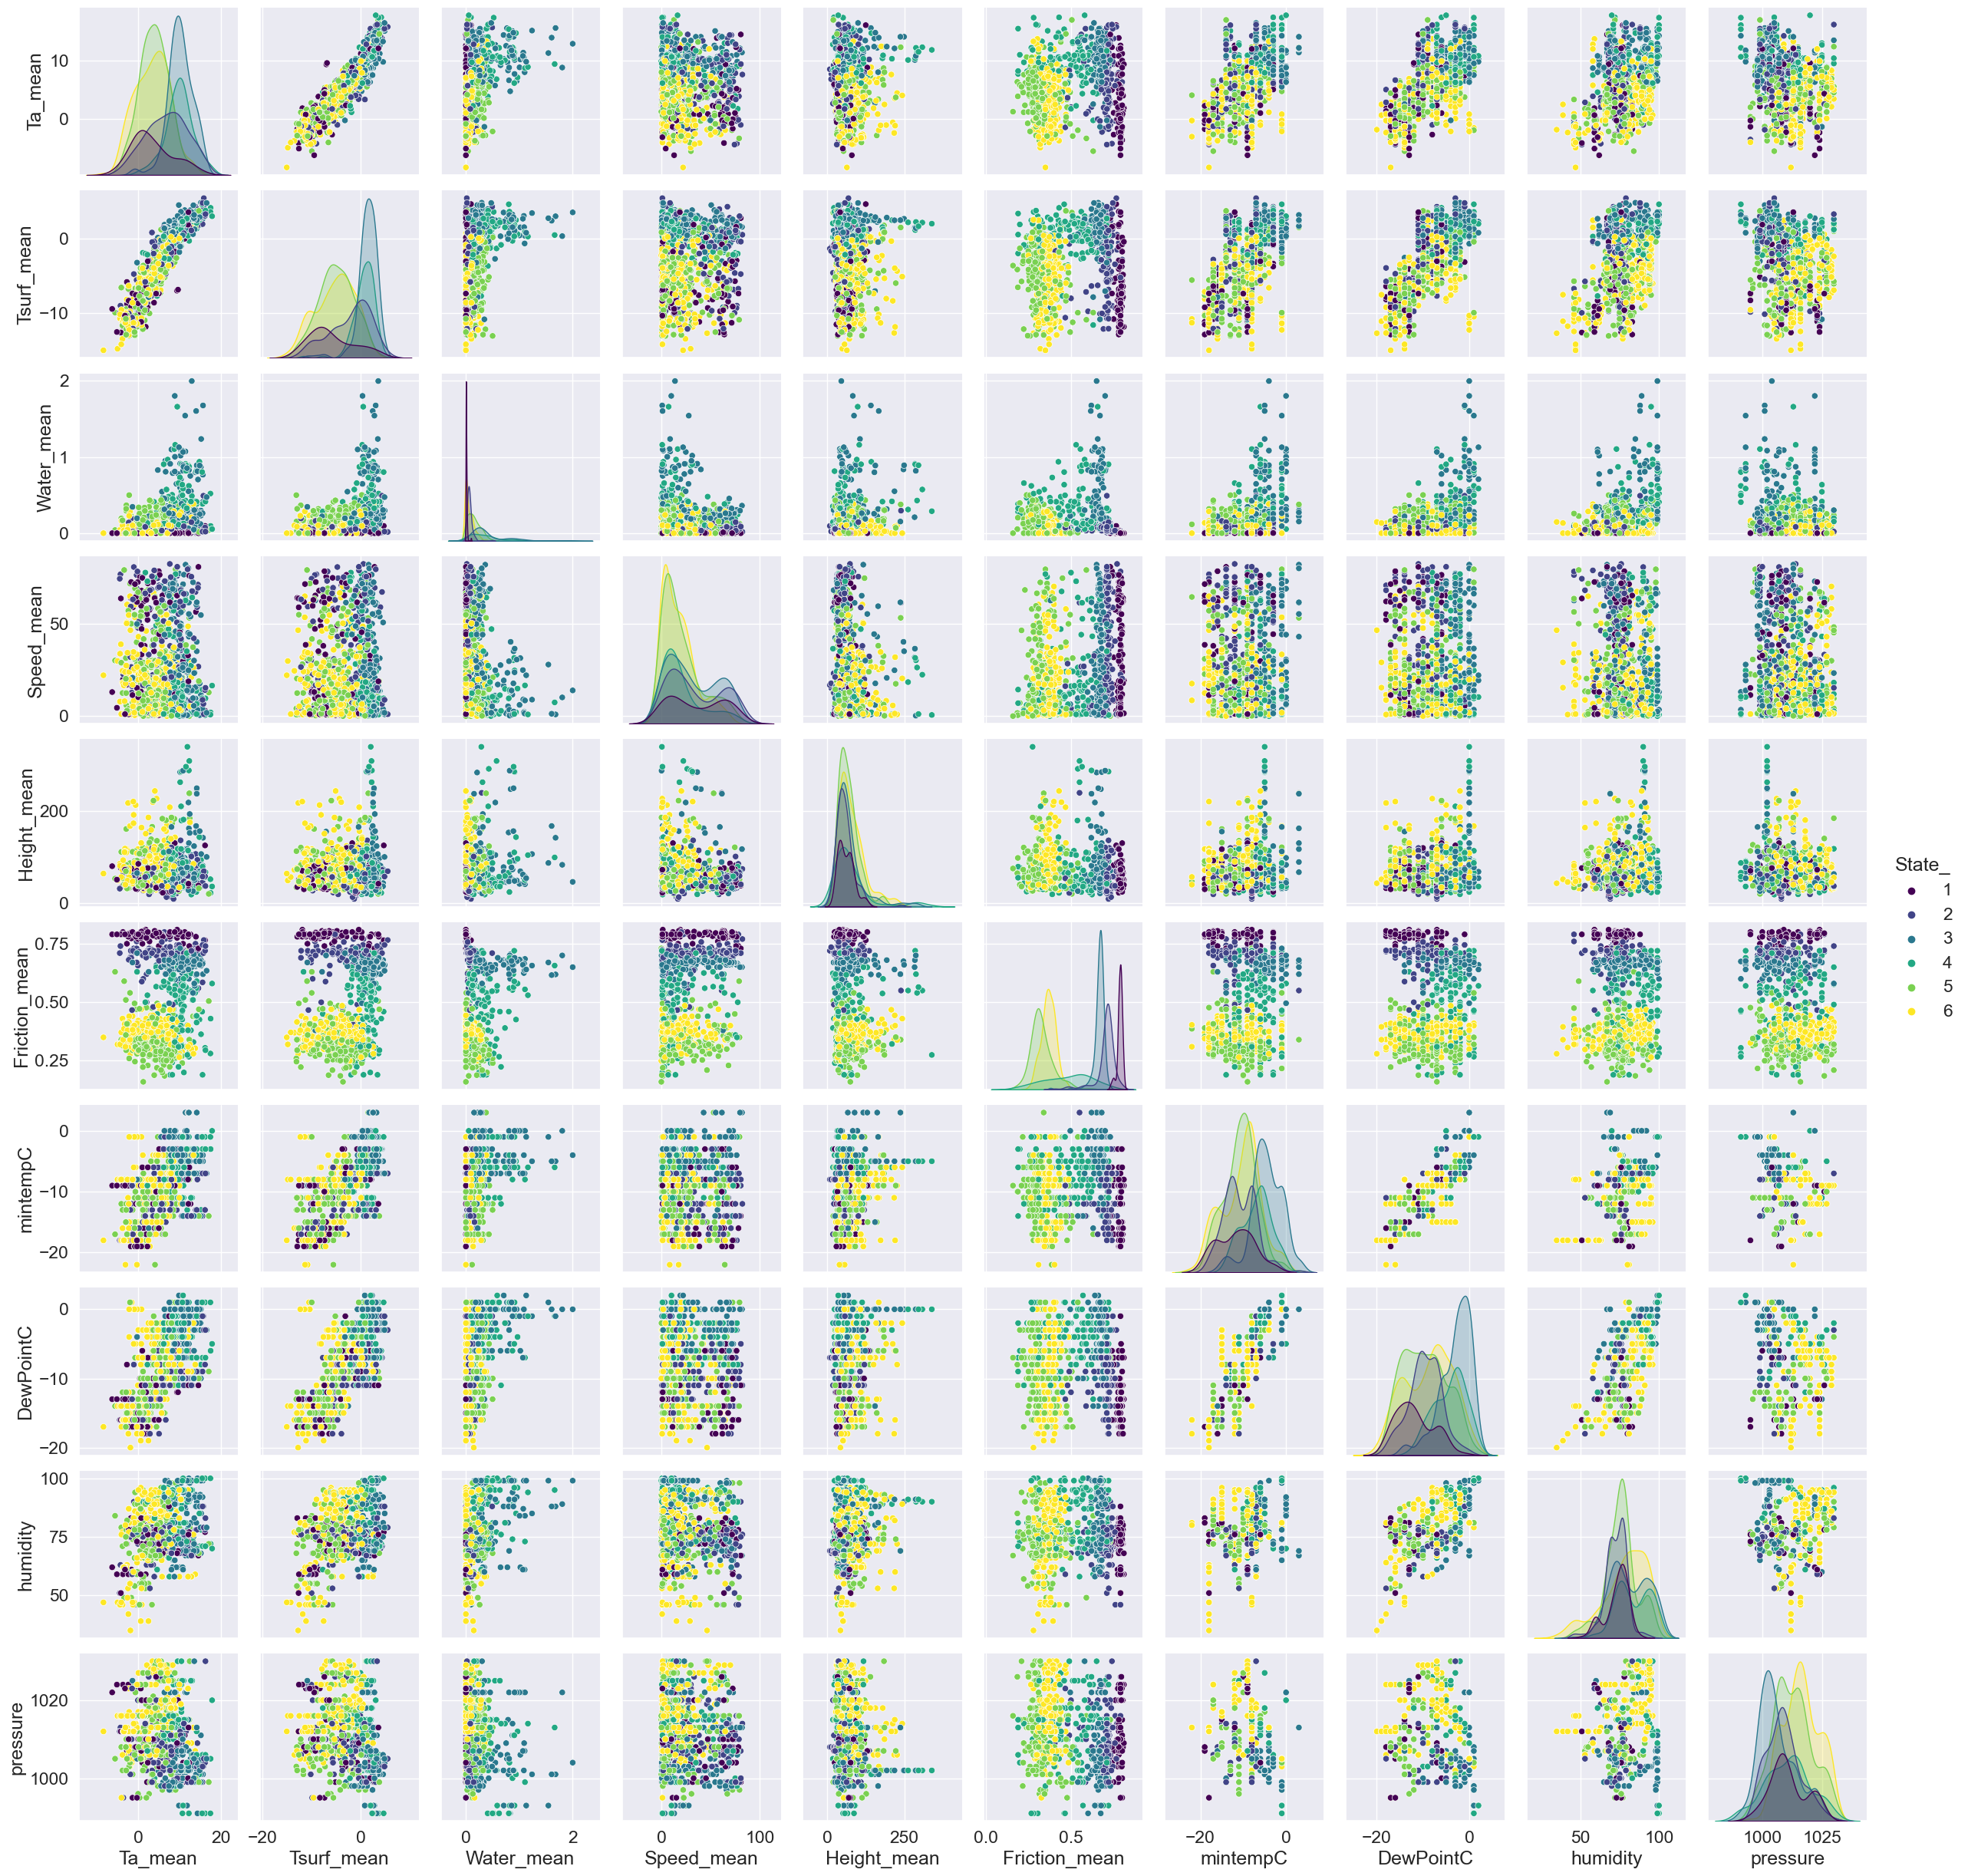
\includegraphics[width=.9\linewidth]{pairplot}
	\label{fig: 4a}
   \end{minipage}\\
\caption{visibility's probability distribution}
\label{fig: 4}
\end{figure}


\begin{table}[!h]
$$
\begin{array}{|c|c|c|c|c|c|c|c|c|c|c|c|}
\hline
\text{visibility} & 0 & 1 & 2 & 3 & 4 & 5 & 6 & 7 & 8 & 9 & 10\\
\hline
p_i & 0.003 & 0.004 & 0.089 & 0.036 & 0.053 & 0.014 & 0.034 & 0.027 & 0.024 & 0.026 & 0.69\\
\hline
\end{array}
$$
\caption{visibility's distribution table}
\label{tab: 1}
\end{table}

Since further we are interested in the construction of a model related to Friction\_mean, it may be useful to have a look at some joint distributions with several continuous features. In figures \ref{fig: 15} and \ref{fig: 16} KDE of joint distributions of Friction\_mean with humidity and Height\_mean correspondingly are presented. 


\begin{figure}[!h]
\centering
   \begin{minipage}{0.7\textwidth}
     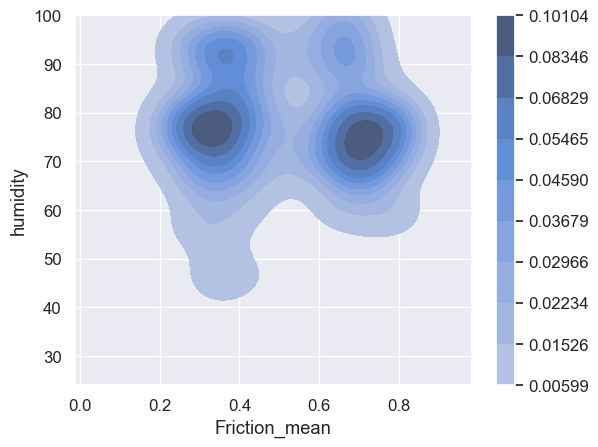
\includegraphics[width=\linewidth]{frihum}
   \end{minipage}
\caption{KDE of Friction\_mean and humidity joint distribution density}
\label{fig: 15}
\end{figure}


\begin{figure}[!h]
\centering
   \begin{minipage}{0.7\textwidth}
     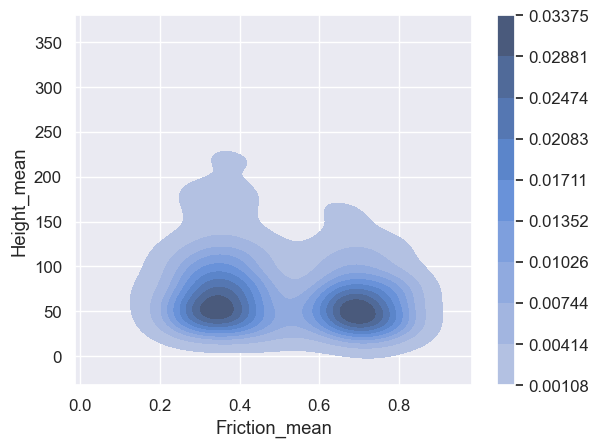
\includegraphics[width=\linewidth]{frihei}
   \end{minipage}
\caption{KDE of Friction\_mean and Height\_mean joint distribution density}
\label{fig: 16}
\end{figure}

\section{Estimation of multivariate mathematical expectation and variance}
\label{sec: est}
Starting from now, we separate the dataset into three ones $D_{l4}, D_{=4}$ and $D_{b4}$ with respect to State\_ $<4$, State\_ $=4$, State\_ $>4$ and emphasize our analysis only on  $D_{l4}$ with the following variables: Friction\_mean, Ta\_mean, Tsurf\_mean,
       Water\_mean, Speed\_mean, Height\_mean, maxtempC, mintempC, totalSnow\_cm,
       sunHour, uvIndex, DewPointC, FeelsLikeC, HeatIndexC,
      WindChillC, WindGustKmph, cloudcover, humidity, precipMM,
       pressure, tempC, visibility, windspeedKmph. In tables \ref{tab: 2} we provide a part of mean vector and a part of covariance matrix estimate~for~$D_{l4}$.

\begin{table}[h]
\tiny
$$
\begin{array}{|c|c|}
\hline
Friction\_mean &      0.702652\\
\hline
Ta\_mean          &   7.521634\\
\hline
Tsurf\_mean       &  -1.397904\\
\hline
Water\_mean       &   0.210166\\
\hline
Speed\_mean        & 33.798909\\
\hline
Height\_mean       & 64.505240\\
\hline
maxtempC          & -2.789346\\
\hline
\end{array}
$$

$$
\begin{array}{|c|c|c|c|c|c|c|c|}
\hline
 & Friction\_mean & Ta\_mean & Tsurf\_mean & Water\_mean & Speed\_mean  & Height\_mean & maxtempC\\
\hline
Friction\_mean & 0.0039 & -0.1088 & -0.1120 & -0.0075 &  0.2216 & -0.2126 & -0.1273\\
\hline
Ta\_mean & -0.1088 & 24.2010 & 20.1588 & 0.5494 & -16.8366 & 27.5351 & 14.1173\\
\hline
Tsurf\_mean & -0.1120 & 20.1588 & 20.1056& 0.5425& -9.8468 & 20.8742 & 15.4006\\
\hline
Water\_mean & -0.0075 & 0.5494 & 0.5425& 0.0901 & -1.7833 & 2.8684 & 0.6905\\
\hline
Speed\_mean  & 0.2216 & -16.8366 & -9.8468 & -1.7833 & 682.6403& -134.7463& -3.7089 \\ 
\hline
Height\_mean & -0.2126& 27.5351 & 20.8742 & 2.8684 &-134.7463 & 1489.7925 & 32.6421 \\
\hline
maxtempC & -0.1273 & 14.1173 & 15.4006 & 0.6905 & -3.7089 & 32.6421& 20.258915\\
\hline
\end{array}
$$

\caption{Parts of mean vector and covariance matrix for $D_{l4}$}
\label{tab: 2}
\end{table}


\section{Non-parametric estimation of conditional distributions, mathematical
expectations and variances}

In figure \ref{fig: 5} KDEs of conditional distributions of Friction\_mean given humidity's bins built on quartiles are illustrated on the left (for subdataset $D_{l4}$). At the same time on the right here are conditional mean (upper graph) and variance kernel estimates (lower graph). The points are colored with respect to State\_.

\begin{figure}[!h]
   \begin{minipage}{.48\textwidth}
     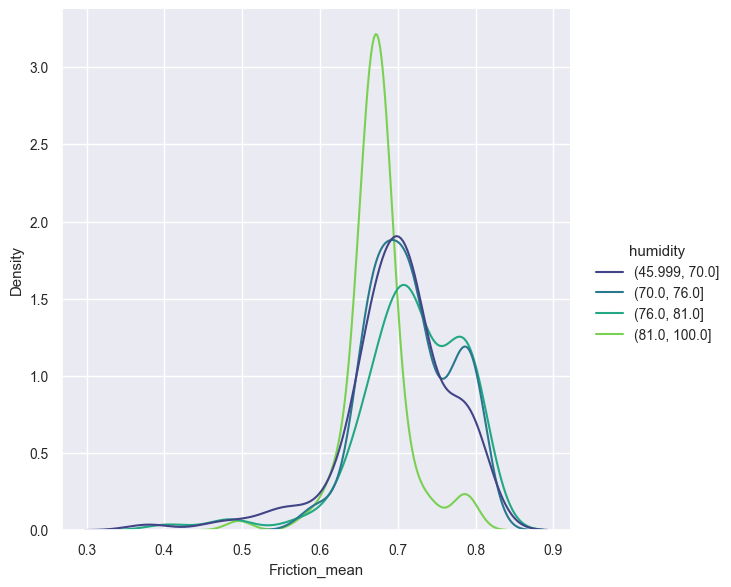
\includegraphics[width=\linewidth]{friction_humiditym}
   \end{minipage} \hfill
\begin{minipage}{.48\textwidth}
     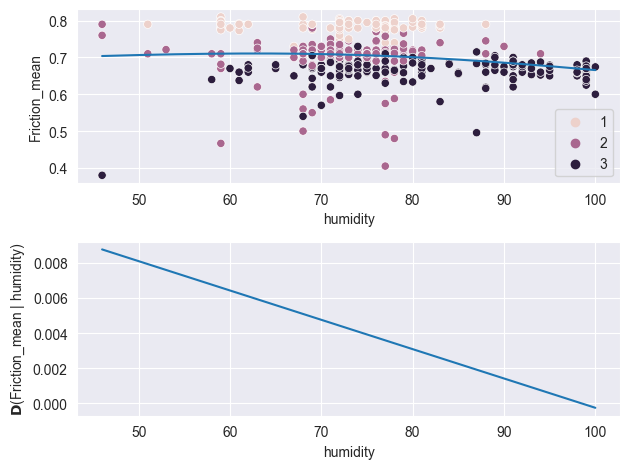
\includegraphics[width=\linewidth]{friction_humidityv}
   \end{minipage}
\caption{Conditional distributions KDEs, mean and variance of Friction\_mean given humidity (or humidity's bins based on quartiles)}
\label{fig: 5}
\end{figure}

In addition, in figure \ref{fig: 6} KDEs of conditional distributions of Friction\_mean given Height\_mean's bins built on quartiles are illustrated (for subdataset $D_{b4}$). On the right here are conditional mean (upper graph) and variance kernel estimates (lower graph). The points are colored with respect to State\_.

\begin{figure}[!h]
   \begin{minipage}{.48\textwidth}
     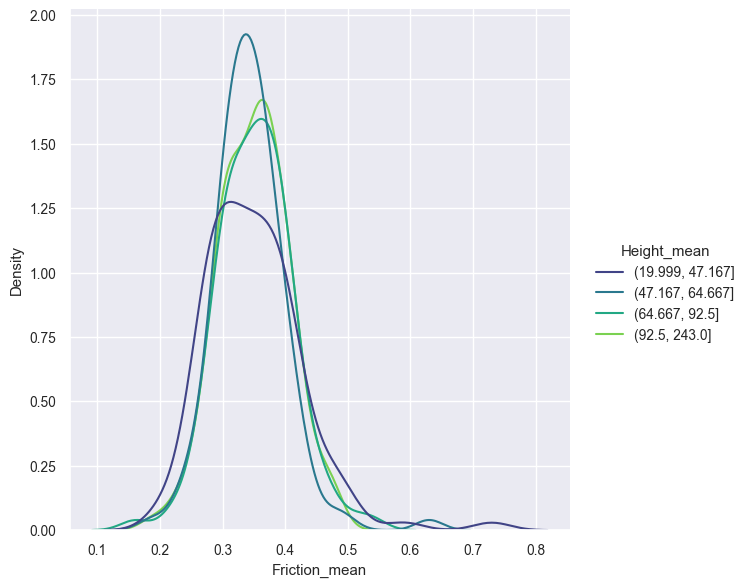
\includegraphics[width=\linewidth]{friction_height}
   \end{minipage} \hfill
\begin{minipage}{.48\textwidth}
     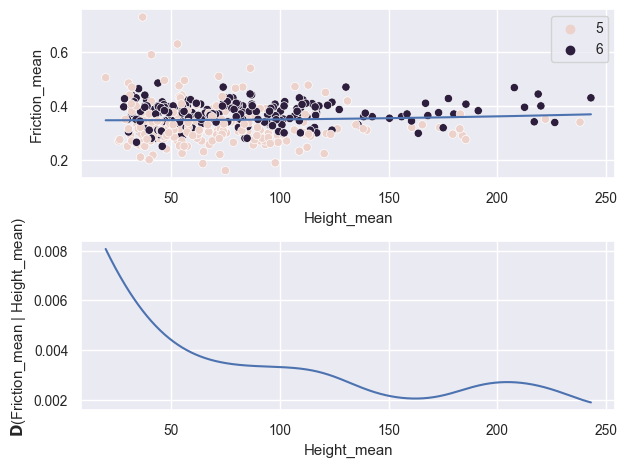
\includegraphics[width=\linewidth]{friction_heightm}
   \end{minipage}
\caption{Conditional distributions KDEs, mean and variance of Friction\_mean given Height\_mean (or Height\_mean's bins based on quartiles)}
\label{fig: 6}
\end{figure}

Conditional variance estimator is obtained from quite simple calculations. If $\mathbf{E}(\xi \mid \eta)$ is a regression of $\xi$ on $\eta$, then $\mathbf{D}(\xi \mid \eta) = \mathbf{E}((\xi - \mathbf{E}(\xi \mid \eta))^2 \mid \eta)$ is a regression of $(\xi - \mathbf{E}(\xi \mid \eta))^2$ on $\eta$.

\section{Estimation of pair correlation coefficients, confidence intervals for them and
significance levels}
\subsection{Theory}
Let $\hat{\rho}_n$ be estimator of $\rho = \rho(\xi, \eta)$ with $(\xi, \eta)^T \sim N(\mu, \Sigma)$. We test the hypothesis $H_0: \rho = 0$. It is known that \[ t = \sqrt{n-2}\frac{\hat{\rho}_n}{\sqrt{1-\hat{\rho}^2_n}} \sim t(n-2) \]
--- a statistic which measures correlation. If our data do not obey Gaussian distribution, then the test utilizes critical values of asymptotic normal distribution $N(0, 1)$ (if n is large enough). It is possible to transform this statistic by $z$-transformation (Fisher):
\[ z = \frac{1}{2} \ln \frac{1+\hat\rho_n}{1-\hat\rho_n},\ z_0 = \frac{1}{2} \ln \frac{1+\rho_0}{1-\rho_0} \]
which implies:
$$ \sqrt{n-3}(z-z_0) \to^d N(0, 1) $$

Given significance level $\alpha$, one can obtain both $p-value$ and $1-\alpha$ asymptotic confidence interval for $z_0$. As soon as we derived the latter, we can find confidence interval for $\rho$ by inverse of $z$-transformation:

\[ z_l < z_0 < z_r \implies 1 - \frac{2}{e^{2z_l}+1} < \rho < 1 - \frac{2}{e^{2z_r}+1} .\] 

\subsection{Results}

We conducted correlation significance analysis of Friction\_mean versus other features chosen in section \label{sec: est} by the aforementioned test on significance level $\alpha = 0.05$. The results are provided in table \ref{tab: 3}.

\begin{table}[!h]
$$
\begin{array}{|c|c|c|c|c|}
\hline
Friction\_mean\ vs & \hat\rho_n & \rho_{left} & \rho_{right} & p-value\\
\hline
DewPointC & -0.4414 & -0.5159 & -0.3603 & 4\text{e-21}\\
\hline
FeelsLikeC & -0.4310 & -0.5064 & -0.3490 & 4\text{e-20}\\
\hline
HeatIndexC & -0.4484 & -0.5223 & -0.3678 & 8\text{e-22}\\
\hline
Height\_mean & -0.0886 & -0.1835 & 0.0080 & 0.0722\\
\hline
Speed\_mean & 0.1364 & 0.0404 & 0.2299& 0.0055\\
\hline
Ta\_mean& -0.3555 & -0.4370 & -0.2682 & 9\text{e-14}\\
\hline
Tsurf\_mean & -0.4017 & -0.4796 & -0.3175 & 2\text{e-17}\\
\hline
Water\_mean & -0.4014 &-0.4793 & -0.3171 & 2\text{e-17}\\
\hline
WindChillC & -0.4310 & -0.5064 & -0.3490 & 4\text{e-20}\\
\hline
WindGustKmph & 0.1404 & 0.0445 & 0.2336 & 0.0043\\
\hline
cloudcover & -0.3011 & -0.3864 & -0.2107 & 4\text{e-10}\\
\hline
humidity & -0.1659 & -0.2582 & -0.0705& 7\text{e-04}\\
\hline
maxtempC & -0.4546 & -0.5279 & -0.3743 & 2\text{e-22}\\
\hline
mintempC & -0.3872 & -0.4663 & -0.3020 & 3\text{e-16}\\
\hline
precipMM & -0.2133 & -0.3035 & -0.1192 & 1\text{e-05}\\
\hline
pressure & 0.1204 & 0.0242 & 0.2144 & 0.0144 \\
\hline
sunHour & 0.0601 & -0.0366 & 0.1557 & 0.2227\\
\hline
tempC & -0.4489 & -0.5227 & -0.3683 & 7\text{e-22}\\
\hline
totalSnow\_cm & -0.1655 & -0.2579 & -0.0701 & 7\text{e-04}\\
\hline
uvIndex & 0.2073 & 0.1131 & 0.2978 & 2\text{e-05}\\
\hline
visibility & 0.2561 & 0.1637 & 0.3441 & 1\text{e-07}\\
\hline
windspeedKmph & 0.1332 & 0.0371 & 0.2267 & 0.0067\\
\hline
\end{array}
$$

\caption{Correlation significance of Friction\_mean vs others test results}
\label{tab: 3}
\end{table}

As one can see, there is no significance of correlation with sunHour and Height\_mean ($p-value > \alpha$) so we omit these features further and use others to build first linear regression model.

\section{Task formulation for regression}
Our purpose is to build regression model for Friction\_mean on data $D_{l4}$ by features Ta\_mean, Tsurf\_mean,
       Water\_mean, Speed\_mean, maxtempC, mintempC, totalSnow\_cm,
      uvIndex, DewPointC, FeelsLikeC, HeatIndexC,
      WindChillC, WindGustKmph, cloudcover, humidity, precipMM,
       pressure, tempC, visibility, windspeedKmph with further selection of predictors and, if any, deleting some observations by means of different statistical tools.

\section{Regression model construction}
\subsection{Model 1}
The first model was built with the aforementioned variables. To check its quality, we look at $R_{adj}^2$ and $MSE$ scores as well as the residuals of the model: their normal probability plot (QQ-plot versus standard normal distribution after standardization).

This model has $R_{adj}^2 \approx 0.233$ and $MSE \approx 0.0028$. The QQ-plot of the residuals is illustrated in figure \ref{fig: 7}. By no means can one treat these residuals as normally distributed so this model was not accepted. 

\begin{figure}[!h]
   \begin{minipage}{\textwidth}
     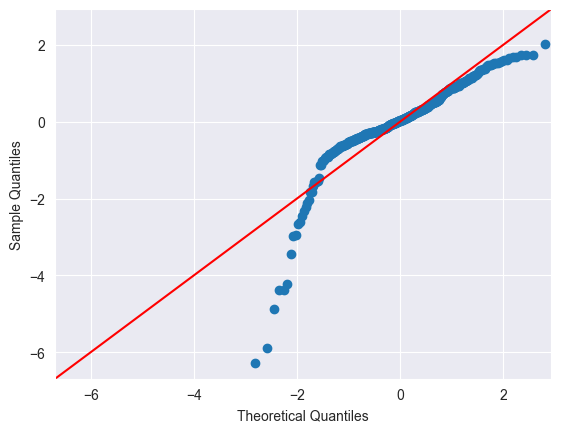
\includegraphics[width=\linewidth]{resqq1}
   \end{minipage}
\caption{Normal probability plot for the residuals of Model 1}
\label{fig: 7}
\end{figure}

\subsection{Multicollinearity and partial correlation analysis}
In order to improve model quality, we decided to look at correlation between our predictors to remove all extra variables which correlate significantly with some others. The heatmap for correlation coefficients between our predictors is demonstrated in \ref{fig: 8}. As has been seen, the whole group of 'temperature' features has strong correlation. We removed all of these variables except Tsurf\_mean as surface temperature closely relates to roads. Furthermore, feature WindGustKmph heavily correlates with windspeedKmph so we also removed the former further. However, the latter is also extra since it replicates feature Speed\_mean but in hourly manner so it is quite discrete. At last, variable visibility is discrete (has 11 unique values) and its distribution is heavily focused on value $10$, thus, we consider interaction with this feature difficult in building regression model and removed it.

\begin{figure}[!h]
   \begin{minipage}{.48\textwidth}
     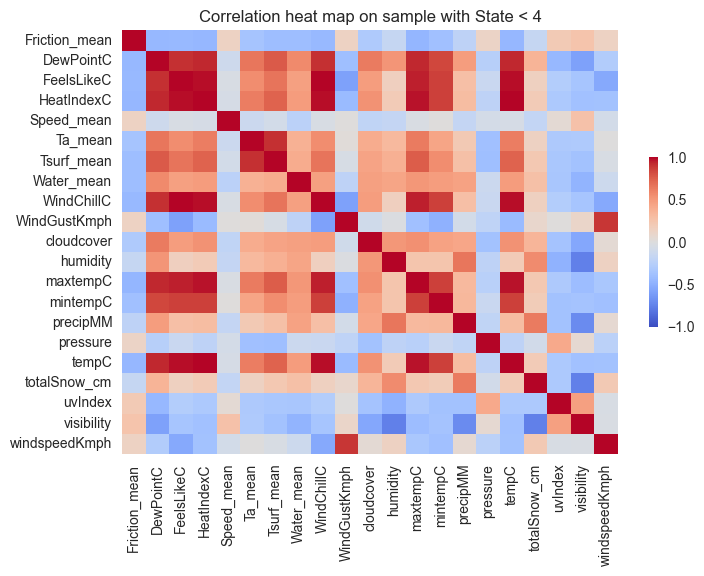
\includegraphics[width=\linewidth]{heatmap}
   \end{minipage} \hfill
\begin{minipage}{.48\textwidth}
     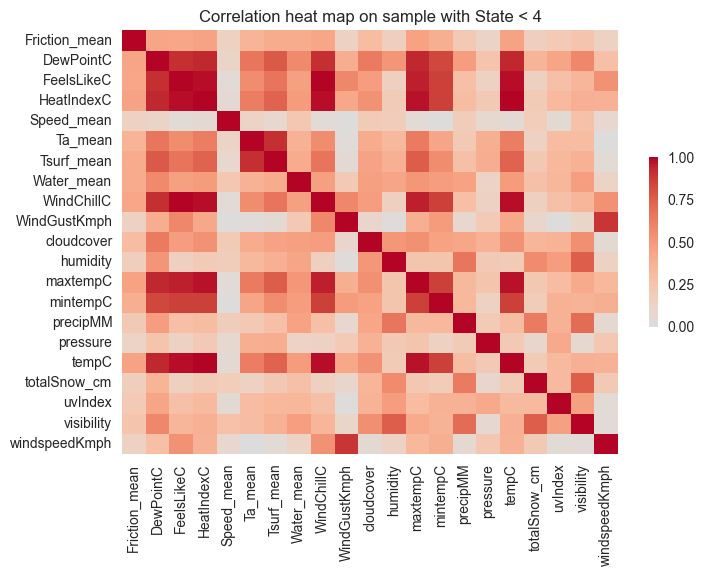
\includegraphics[width=\linewidth]{heatmap1}
   \end{minipage}
\caption{Heatmap for correlation coefficients: one is colored depending on the sign of the correlation, another is colored by absolute values of correlation coefficients}
\label{fig: 8}
\end{figure}

Also we analyzed partial correlations between our target variable Friction\_mean and others to find potential predictors which correlates with target even if the influence of other variables is neutralized. 

Partial correlation measures correlation of two variables if influence of other variables is removed:
\begin{align*} 
\rho(\xi, \eta \mid \alpha_1, \dots, \alpha_n) &= \rho(\xi - \widetilde{\xi}, \eta - \widetilde{\eta})\\
\widetilde{\xi} &= \arg \min_{\xi^* \in K} \mathbf{E} (\xi - \xi^*)^2 \\
\widetilde{\eta} &= \arg \min_{\eta^* \in K} \mathbf{E} (\eta - \eta^*)^2\\
K &= \{a_0 + a_1 \alpha_1 + \dots + a_n \alpha_n\}\\
\end{align*}

In figure \ref{fig: 9} one can see partial correlation heatmap. It is evident that no variable has own separate influence on the target so we have to deal with all variables selected above.

\begin{figure}[!h]
\centering
   \begin{minipage}{0.7\textwidth}
     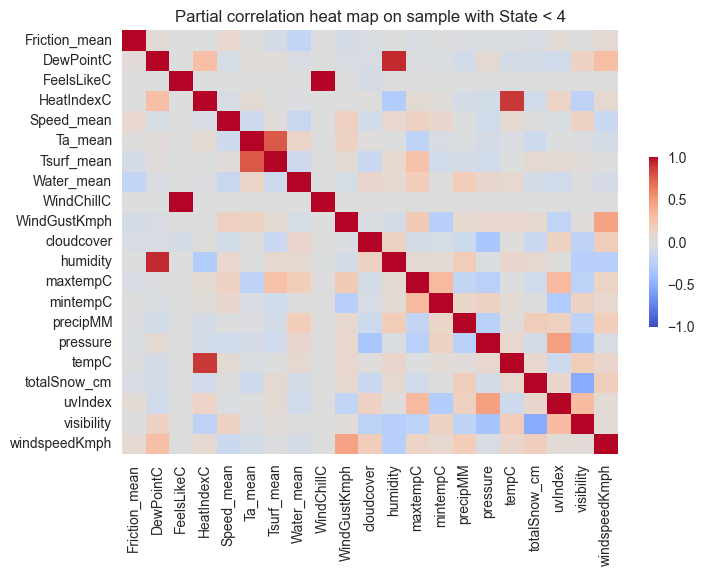
\includegraphics[width=\linewidth]{parheatmap}
   \end{minipage}
\caption{Partial correlation heatmap}
\label{fig: 9}
\end{figure}

As a result of variables selection, we further work with the following variables: Tsurf\_mean,
       Water\_mean, Speed\_mean, totalSnow\_cm,
       uvIndex, DewPointC, cloudcover, humidity, precipMM,
      pressure.

\subsection{Outlier with respect to distribution removal}
Besides, we decided to remove outliers using histogram of the target variable and Mahalanobis distance on the regressors. From graph \ref{fig: 10} one can conclude that observations with Friction\_mean $< 0.5$ may be treated as outliers since at least they heavily influence on regression. 
\begin{figure}[!h]
\centering
   \begin{minipage}{0.7\textwidth}
     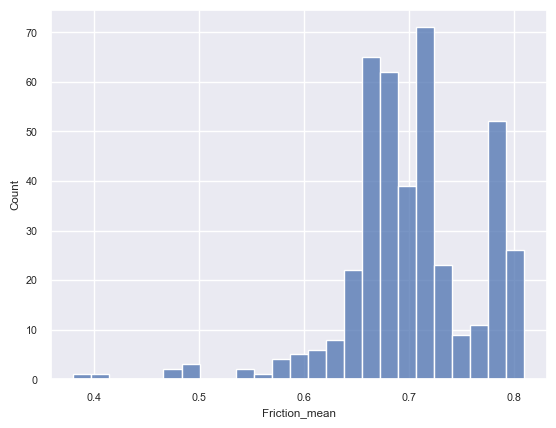
\includegraphics[width=\linewidth]{friction_dist}
   \end{minipage}
\caption{Friction\_mean histogram, State\_ $<4$}
\label{fig: 10}
\end{figure}

\subsubsection{Mahalanobis' distance}
Suppose $S$ is a positive definite $d\times d$ matrix. The Mahalanobis' distance between two points $x, y \in \mathbf{R}^d$ with these matrix is defined as follows:
\[ d^2_M(x,y; S) = (x-y)S^{-1}(x-y)^{T}. \]

If $\xi \sim N(\mu, \Sigma)$, then $d^2(\xi, \mu; \Sigma) \sim \chi^2(d)$. Using these information one can construct statistical test for outliers detection if data are normal, otherwise, one can just analyze the graph of Mahalanobis' distribution of all observations with respect to empirical distribution.

As our data are not normal, we analyzed the Mahalanobis' distance graph \ref{fig: 11}. We treat the observations with $d_M > 8$ as explicit outliers so we remove them in further analysis as well as the observations with Friction\_mean $< 0.5$.
\begin{figure}[!h]
\centering
   \begin{minipage}{0.7\textwidth}
     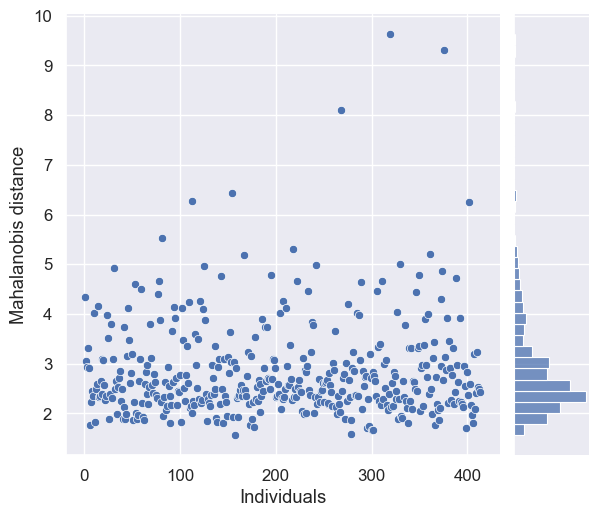
\includegraphics[width=\linewidth]{mahalanobis}
   \end{minipage}
\caption{Mahalanobis' distance jointplot}
\label{fig: 11}
\end{figure}

\subsection{Model 2}
After multicollinearity analysis and distribution outliers analysis, we trained linear regression model with aforementioned features. Its $R^2_{adj} \approx 0.408$ and $MSE = 0.0017$ which are significantly better than of the Model 1. However, the residuals' distribution is far from being normal as shown in the QQ-plot \ref{fig: 12} 
\begin{figure}[!h]
\centering
   \begin{minipage}{0.7\textwidth}
     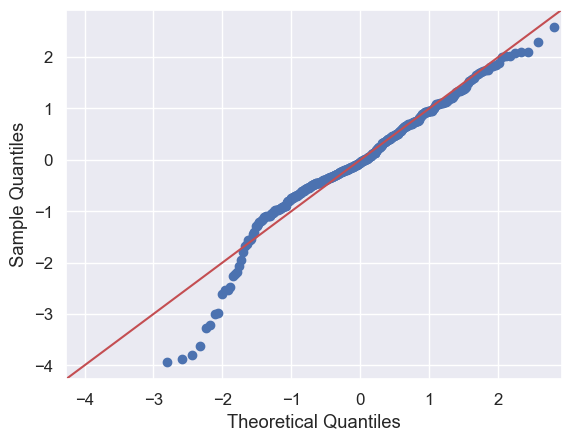
\includegraphics[width=\linewidth]{resqq2}
   \end{minipage}
\caption{Normal probability plot for the residuals of Model 2}
\label{fig: 12}
\end{figure}

Consider a significance test of Model 2 regression coefficients. Its result on significance level $\alpha = 0.05$ are presented in table \ref{tab: 4} .
\begin{table}[!h]
$$
\begin{array}{|c|c|c|c|c|c|c|}
\hline
 & coef & std\ err & t & P>|t| & [0.025 & 0.975]\\
\hline
intercept & 0.6627 & 0.33 & 2.007 & 0.045 & 0.014 & 1.312\\
\hline
Tsurf\_mean & -0.0044 & 0.001 & -7.900 & \approx 0 & -0.006 & -0.003\\
\hline
Water\_mean & -0.0641 & 0.009 & -6.952 & \approx 0 & -0.082 & -0.046\\
\hline
Speed\_mean & 3\text{e-06} & 8\text{e-05} & 0.037 & 0.971 & \approx -0 & \approx 0\\
\hline
totalSnow\_cm & -0.0005 & 0.001 & -0.821 & 0.412 & -0.002 & 0.001\\
\hline
uvindex & 0.0093 & 0.005 & 1.819 & 0.070 & -0.001 & 0.019\\
\hline
cloudcover & -0.0002 & 9\text{e-05} & -1.939 & 0.053 & \approx -0 & 2\text{e-06}\\
\hline
humidity & 0.0009 & \approx 0 & 3.002 & 0.003 & \approx 0 & 0.002\\
\hline
precipMM & -0.0081 & 0.010 & -0.788 & 0.431 & -0.0028 & 0.012\\
\hline
pressure & -2\text{e-05} & \approx 0 & -0.064 & 0.949 & -0.001 & 0.001 \\
\hline
\end{array}
$$

\caption{Regression coefficients significance test results: coefficients, their standard error, test statistic value, p-values and 95\% confidence intervals}
\label{tab: 4}
\end{table}

One can infer that Speed\_mean, totalSnow\_cm, uvindex, precipMM and pressure have no evidence to be proved significant so we decided to remove these feature. In spite of $p-value$ of the coefficient of cloudcover being a bit above $0.05$, we did not remove it in further analysis.

So, the left features are Tsurf\_mean, Water\_mean, cloudcover and humidity (and intercept!).

\subsection{Outliers with respect to regression analysis}
Using the aforementioned features, we analyzed outliers with respect to regression (i.e. observations with high leverage).

\subsubsection{Cook's distance}

Let $y = X w + \varepsilon$, $w \in \mathbb{R}^{p+1}$ and $\varepsilon \sim N(0, \sigma^2 I)$. It is evident that $\widehat{w}= \widehat{w}_{OLS} = (X^TX)^{-1}X^Ty$ and $\widehat{y} = X(X^TX)^{-1}X^Ty = Hy$.

Residual for $y_i$: $r_i = y_i - \widehat{y_i}$, deleted residual: $r_i^{(i)} = y_i - \widehat{y_i}^{(i)}$, where $\widehat{y_i}^{(i)}$ --- estimator of $y_i$ with regression built on data without $i-$th individual.

It follows from the definition that $\mathbb{D}r_i = \sigma^2(1-h_{ii})$ and then $\frac{r_{i}}{\widehat{\sigma}\sqrt{1-h_{ii}}}$ --- studentized residual, $\widehat{\sigma^2}=\frac{1}{n-p}\sum_{k=1}^n(y_k-\widehat{y_k})^2$.

Cook's distance from $i$-th individual to regression is:
$$ D_i = \frac{\sum_{k=1}^n(\widehat{y_k}-\widehat{y_k}^{(i)})^2}{p\widehat{\sigma^2}} = \frac{(y_i-\widehat{y_i})^2}{p\widehat{\sigma^2}} \frac{h_{ii}}{(1-h_{ii})^2} $$

There is a rule-of-thumb: the observations with $D_i > \frac{4}{n}$ are believed to be outliers \cite{fox91}.

In our case, the graph of Cook's distance is demonstrated in figure \ref{fig: 13} where the threshold is approximately equal to $0.01$. We treat these observations as outliers since they have significant leverage for regression construction.

\begin{figure}[!h]
\centering
   \begin{minipage}{0.7\textwidth}
     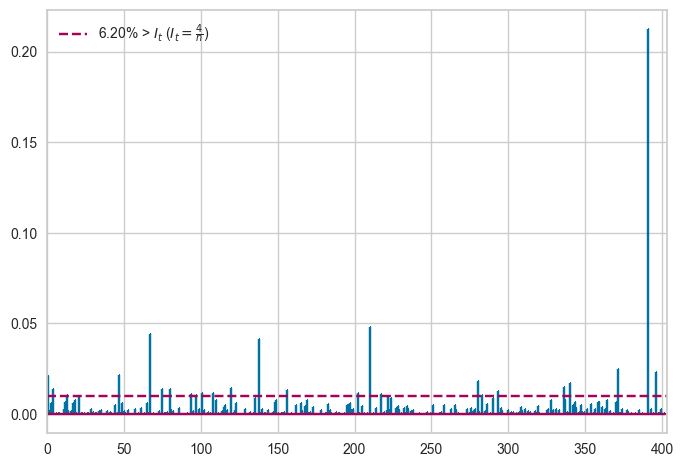
\includegraphics[width=\linewidth]{cook}
   \end{minipage}
\caption{Cook's distance plot}
\label{fig: 13}
\end{figure}

\subsection{Model 3}
The model built on the data with aforementioned features has $R^2_{adj} \approx 0.565$ and $MSE \approx 0.001$. These values are better than those of Model 2. If one looks at the QQ-plot (fig. \ref{fig: 14}) of the regression residuals, they can treat the residuals as practically normal.

\begin{figure}[!h]
\centering
   \begin{minipage}{0.7\textwidth}
     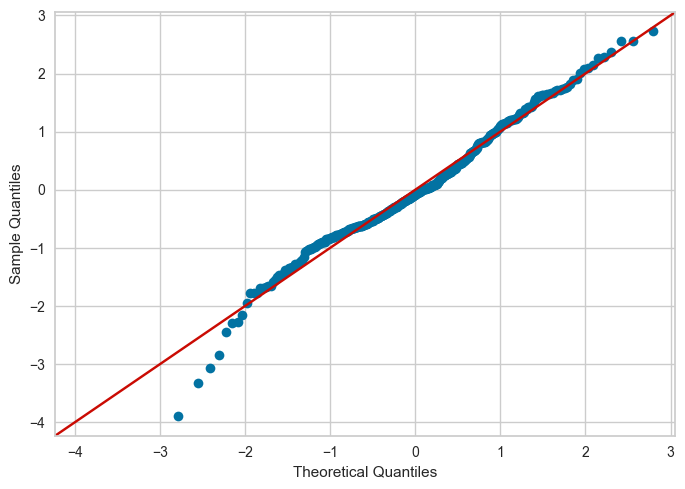
\includegraphics[width=\linewidth]{res4}
   \end{minipage}
\caption{Normal probability plot for the residuals of Model 3}
\label{fig: 14}
\end{figure}

 We consider this model as final one. Its description in terms of coefficients significance are listed in table \ref{tab: 5}.

\begin{table}[!h]
$$
\begin{array}{|c|c|c|c|c|c|c|}
\hline
 & coef & std\ err & t & P>|t| & [0.025 & 0.975]\\
\hline
intercept & 0.7001 & 0.014 & 48.744 & \approx 0 & 0.672 & 0.728\\
\hline
Tsurf\_mean & -0.0054 & \approx 0 & -10.965 & \approx 0 & -0.006 & -0.004\\
\hline
Water\_mean & -0.0854 & 0.008 & -10.136 & \approx 0 & -0.102 & -0.069\\
\hline
cloudcover & -0.0001 & 7\text{e-05} & -2.017 & 0.044 & \approx -0 & -3.6\text{e-06}\\
\hline
humidity & 0.0004 & \approx 0 & 1.826 & 0.069 & \approx -3\text{e-05} & 0.001\\
\hline
\end{array}
$$

\caption{Regression coefficients significance test results on Model 3: coefficients, their standard error, test statistic value, p-values and 95\% confidence intervals}
\label{tab: 5}
\end{table}

\section{Appendix}
The Python notebook related to the aforementioned calculations is presented in Github \cite{repogithub}.

{\small \bibliography{biblio}}
\bibliographystyle{gost2008}

\end{document}